\documentclass[10pt,letterpaper]{article} 
\usepackage{tikz}
\usepackage{toolsper}
%\usepackage{graphicx}‎‎
%\usefonttheme{serif}‎
%\usepackage{ptext}‎
%\usepackage{xepersian}
%\settextfont{B Nazanin}
\usepackage{lipsum}
\setlength{\parindent}{0pt}
\setlength{\parskip}{1em}
\newcommand{\pf}{$\blacksquare$}
\newcommand{\EX}{\Bbb E}
\newcommand{\nl}{\newline\newline}
\newcounter{QuestionNumber}
\setcounter{QuestionNumber}{1}

\newcommand{\wid}{40mm}
%\newcommand

\newcommand{\Q}{
\textbf{
سوال \theQuestionNumber)
}
\stepcounter{QuestionNumber}
}
\begin{document}
\large
\begin{center}
به نام زیبایی

پاسخ تمرینات سری یازدهم سیگنال ها و سیستم ها
\hl
\end{center}
\Q

الف) از آنجا که در قطب ها مقدار پاسخ فرکانسی به سمت مقدار نامحدود میل می کند (و یا وجود ندارد)، بنا به تعریف ناحیه همگرایی (که باید مقدار پاسخ فرکانسی موجود و محدود باشد)، این ناحیه نمی تواند شامل هیچ قطبی باشد.

ب) ناحیه‌ی همگرایی تبدیل لاپلاس 
$
x(t)+y(t)
$
 حداقل شامل 
$
R_1\cap R_2
$
 خواهد بود که 
$
R_1
$
 ناحیه‌ی همگرایی تبدیل لاپلاس 
$
x(t)
$
 و 
$
R_2
$
ناحیه‌ی همگرایی تبدیل لاپلاس
$
y(t)
$
 است؛ زیرا در اشتراک این دو ناحیه، هر دو تبدیل لاپلاس
$
X(s)
$
 و 
$
Y(s)
$
 وجود دارند. با این حال، اطلاعات بیشتری نمی توان داد؛ زیرا اصل سیگنال ها تعیین کننده اند؛ به طور مثال اگر دو سیگنال قرینه ی هم باشند (یا دستکم به گونه ای باشند که خارج از یک بازه ی محدود مقدار یکدیگر را خنثی کنند)، ناحیه همگرایی تمام صفحه مختلط خواهد بود.

\Q

می دانیم برای سیگنال
$
x(t)=e^{-at}u(t)
$
:
\qn{
X(s)&=\int_{-\infty}^\infty x(t)e^{-st}dt
\\&=\int_{-\infty}^\infty e^{-at}e^{-st}u(t)dt
\\&=\int_{0}^\infty e^{-at}e^{-st}u(t)dt
\\&=\int_{0}^\infty e^{-at}e^{-st}dt
\\&=\int_{0}^\infty e^{-(a+s)t}dt
\\&={1\over a+s}\quad,\quad \Re\{s\}>-\Re\{a\}
}{}
همچنین برای سیگنال 
$
x(t)=e^{-at}u(-t)
$
:
\qn{
X(s)&=\int_{-\infty}^\infty x(t)e^{-st}dt
\\&=\int_{-\infty}^\infty e^{-at}e^{-st}u(-t)dt
\\&=\int_{-\infty}^0 e^{-at}e^{-st}u(t)dt
\\&=\int_{-\infty}^0 e^{-at}e^{-st}dt
\\&=\int_{-\infty}^0 e^{-(a+s)t}dt
\\&=-{1\over a+s}\quad,\quad \Re\{s\}<-\Re\{a\}
}{}
بنابراین

الف)
$$
e^{-2t}u(t)+e^{-3t}u(t)\iff {1\over s+2}+{1\over s+3}\quad,\quad \Re\{s\}>-2
$$

ب)
$$
e^{t}u(-t)+u(t)\iff -{1\over s+1}+{1\over s}={1\over s^2+s}\quad,\quad 0<\Re\{s\}<1
$$

پ)
$$
x(t)={e^{(1+1j)t}-e^{(1-1j)t}\over 2j}u(-t)+e^{2t}u(t)
$$
از آنجا که ناحیه همگرایی تبدیل لاپلاس 
$
e^{2t}u(t)
$
 برابر 
$
\Re\{s\}>2
$
 و ناحیه همگرایی تبدیل لاپلاس 
$
{e^{(1+1j)t}-e^{(1-1j)t}\over 2j}u(-t)
$
 برابر 
$
\Re\{s\}<1
$
بوده و این دو ناحیه همگرایی هیچ اشتراکی با هم ندارند، در نتیجه سیگنال حاصل جمع، تبدیل لاپلاس ندارد.

ت)
$$
X(s)={1\over s+1}-{1\over s-1}={-2\over s^2-1}\quad,\quad -1<\Re\{s\}<1
$$

ث)
$$
x(t)=te^{-|t|}=t(e^{-t}u(t)+e^{t}u(-t))=te^{-t}u(t)+te^{t}u(-t)
$$
در نتیجه بر طبق خاصیت
$$
tz(t)\iff -Z'(s)
$$
خواهیم داشت:
$$
X(s)=-{d\over ds}{1\over s+1}+{d\over ds}{1\over s-1}={1\over (s+1)^2}-{1\over (s-1)^2}\quad,\quad -1<\Re\{s\}<1
$$

\Q

الف)
\qn{
X(s)&={1\over s^2+9}
\\&={1\over (s+3j)(s-3j)}
\\&={A\over s-3j}+{B\over s+3j}
\\&={{1\over 6j}\over s-3j}+{-{1\over 6j}\over s+3j}
}{}
در نتیجه
$$
x(t)={1\over 6j}(e^{3jt}-e^{-3jt})u(t)={1\over 3}\sin 3tu(t)
$$

ب)
\qn{
X(s)&={s\over s^2+9}
\\&={s\over (s+3j)(s-3j)}
\\&={A\over s-3j}+{B\over s+3j}
\\&={{1\over 2}\over s-3j}+{{1\over 2}\over s+3j}
}{}
در نتیجه
$$
x(t)=-{1\over 2}(e^{3jt}+e^{-3jt})u(-t)=-\cos 3t u(-t)
$$

پ) 
\qn{
X(s)&={s+1\over s^2+5s+6}
\\&={s+1\over (s+2)(s+3)}
\\&={A\over s+2}+{B\over s+3}
\\&=-{1\over s+2}+{2\over s+3}
}{}
بنابراین
$$
x(t)=2e^{-3t}u(t)+e^{-2t}u(-t)
$$
ت)
\qn{
X(s)&={s^2-s+1\over (s+1)^2(s+2)}
\\&={A_1\over s+1}+{A_2\over (s+1)^2}+{B\over s+2}
}{}
که در آن
\qn{
&A_1=\lim_{s\to -1}{d\over ds}(s+1)^2X(s)=-6
\\&A_2=\lim_{s\to -1}(s+1)^2X(s)=3
\\&B=\lim_{s\to -1}(s+2)X(s)=7
}{}
بنابرابن
$$
x(t)= 6e^{-t}u(-t)-3te^{-t}u(-t)-7e^{-2t}u(-t)
$$

\Q

الف) از آنجا که سیگنال 
$
x(t)e^{-3t}
$
 دارای تبدیل لاپلاس 
$
X(s+3)
$
است، این شرط نتیجه می دهد که مقدار 
$
X(3+j\omega)
$
محدود است و درنتیجه ناحیه همگرایی
$
X(s)
$
شامل خط
$
\Re\{s\}=3
$
 خواهد بود. بنابراین شکل های الف تا ت، به ترتیب دارای نواحی همگرایی زیر خواهند بود:
\qn{
& \Re\{s\}>2
\\& \Re\{s\}>-2
\\& \Re\{s\}>2
\\& \text{تمام صفحه‌ی مختلط}
}{}
ب) می دانیم
$
x(t)*e^{-t}u(t)
$
زمانی دارای تبدیل لاپلاس 
$
{X(s)\over s+1}
$
 است که نواحی همگرایی تبدیل لاپلاس های سیگنال های 
$
x(t)
$
 و 
$
e^{-t}u(t)
$
اشتراک داشته باشند. از آنجا که ناحیه همگرایی تبدیل لاپلاس 
$
e^{-t}u(t)
$
 برابر 
$
\Re\{s\}>-1
$
بوده و 
$
X(s)
$
 یک قطب در 
$
s=-1
$
 دارد، بنابراین مشابه قسمت قبل، باید مقدار 
$
X(j\omega)\over 1+j\omega
$
 وجود داشته و محدود باشد و شکل های الف تا ت، به ترتیب دارای نواحی همگرایی زیر خواهند بود:
\qn{
& -2<\Re\{s\}<2
\\& -2<\Re\{s\}
\\& \Re\{s\}<2
\\& \text{تمام صفحه‌ی مختلط}
}{}
پ) مطابق این شرط، ناحیه همگرایی تبدیل لاپلاس 
$
x(t)
$
 باید شامل 
$
s=-\infty
$
 باشد؛ بنابراین شکل های الف تا ت، به ترتیب دارای نواحی همگرایی زیر خواهند بود:
\qn{
& \Re\{s\}<-2
\\& \Re\{s\}<-2
\\& \Re\{s\}<2
\\& \text{تمام صفحه‌ی مختلط}
}{}
پ) مطابق این شرط، ناحیه همگرایی تبدیل لاپلاس 
$
x(t)
$
 باید شامل 
$
s=\infty
$
 باشد؛ بنابراین شکل های الف تا ت، به ترتیب دارای نواحی همگرایی زیر خواهند بود:
\qn{
& \Re\{s\}>2
\\& \Re\{s\}>-2
\\& \Re\{s\}>2
\\& \text{تمام صفحه‌ی مختلط}
}{}
\Q

از شرط اول نتیجه می شود که 
$
X(s)
$
 باید به فرم 
$
{P(s)\over(s+a)(s+b)}
$
باشد. از شرط دوم، چندجمله ای 
$
P(s)
$
 نباید دارای ریشه باشد؛ در این صورت:
$$
P(s)=A\ne 0
$$
به کمک شرط سوم:
$$
X(s)={A\over (s+1-j)(s+b)}
$$
از شرط پنجم خواهیم داشت:
$$
A=8(1-j)b
$$
تا اینجا حل سوال کامل است؛ اما اگر سیگنال را حقیقی فرض کنیم، آنگاه مزدوج مختلط قطب  $
-1+j
$
 یعنی در 
$
-1-j
$
 نیز قطب خواهیم داشت که باعث می شود:
$$
A=16
$$
بنابراین
$$
X(s)={16\over s^2+2s+2}
$$
و از آنجا که ناحیه همگرایی
$
X(s)
$
شامل 
$
\Re\{s\}=-2
$
 نیست، بنابراین
$$
\text{ROC}: \qquad \Re\{s\}>-1
$$

\Q

از شرط 4 نتیجه می شود که 
$
(s^2+2s+2)H(s)
$
 نباید دارای قطب جایی غیر از $s=0$ باشد؛ بنابراین 
$
H(s)
$
 حداکثر در 
$
s=-1+j
$
(ساده) یا 
$
s=-1-j
$
(ساده) یا 
$
s=0
$
 قطب خواهد داشت. از طرفی چون سیستم پایدار است، ناحیه همگرایی آن شامل محور $j\omega$ بوده و در نتیجه سیستم در $s=0$ نیز قطب ندارد.

از شرط 2 نتیجه می شود که تبدیل لاپلاس خروجی یعنی 
$
{H(s)\over s}
$
 دارای قطبی روی محور $j\omega$ نیست و بنابراین 
$
H(s)
$
باید دارای صفری در 
$
s=0
$
باشد. از طرفی طبق شرط 3، خروجی با تبدیل لاپلاس 
$
-{H(s)\over s^2}
$
 باید دارای قطبی روی محور $j\omega$ باشد که این الزام می کند که $H(s)$ باید دارای صفر ساده در $s=0$ باشد. به کمک شرط 5، می توان گفت جایگذاری مقدار $s=\infty$ باعث می شود مقدار $H(s)$ صفر می شود که این مهم، نشان می دهد که درجه ی صورت $H(s)$ از مخرج آن کمتر است. چون در صورت، یک ریشه در $s=0$ داریم، درجه ی مخرج باید از 2 بیشتر یا مساوی باشد. از طرفی، وجود قطب های $
s=-1+j
$
و
$
s=-1-j
$
نتیجه می گیریم که درجه ی مخرج از 2 بیشتر نیست؛ پس نتیجه می گیریم که درجه ی صورت و مخرج به ترتیب برابر 1 و 2 است. تا اینجا داریم:
$$
H(s)=A{s\over (s+1-j)(s+1+j)}={As\over s^2+2s+2}
$$
در نهایت از شرط 1 خواهیم داشت:
$$
A=1
$$
بنابراین:
$$
H(s)={s\over s^2+2s+2}\quad,\quad \Re\{s\}>-1
$$
\Q

می دانیم
$$
|H(j\omega)|={\text{
حاصل ضرب فاصله از صفر ها
}
\over
\text{
حاصل ضرب فاصله از قطب ها
}
}
$$
طبق رابطه‌ی فوق، به طور شهودی اندازه‌ی پاسخ فرکانسی در نزدیکی فرکانس قطب ها به سمت بینهایت و در نزدیکی فرکانس صفرها به صمت صفر میل میکند. بنابراین:
\begin{figure}[h!]
\centering
%%%%%%%%%%%%%%%%%%%%%
\begin{subfigure}{0.49\textwidth}
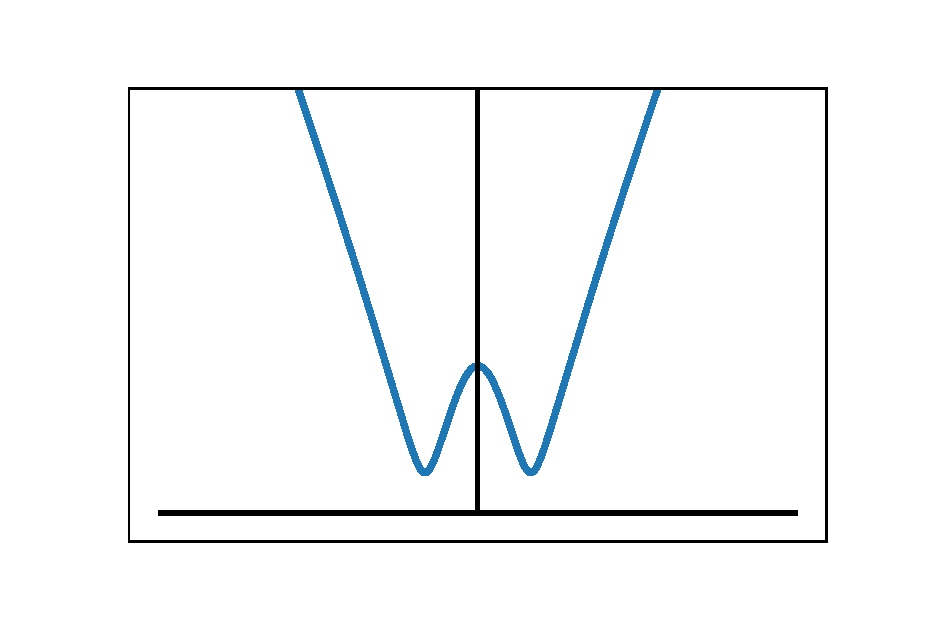
\includegraphics[width=80mm]{PSol10_Q7_zp_2.eps}
\caption{
شکل 1
}
\end{subfigure}
%%%%%%%%%%%%%%%%%%%%%
\begin{subfigure}{0.49\textwidth}
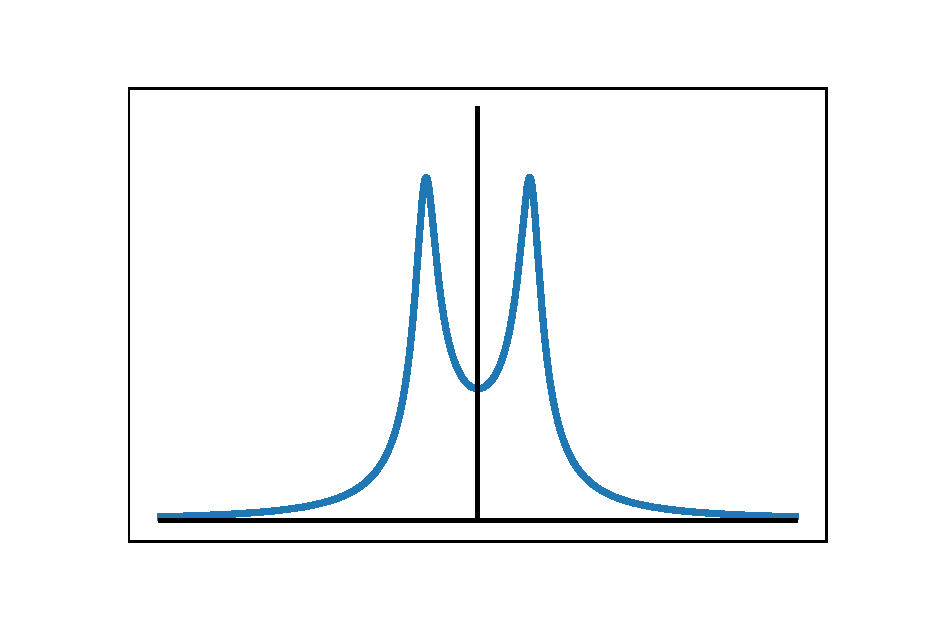
\includegraphics[width=80mm]{PSol10_Q7_zp_1.eps}
\caption{
شکل 2
}
\end{subfigure}
%%%%%%%%%%%%%%%%%%%%%
\begin{subfigure}{0.49\textwidth}
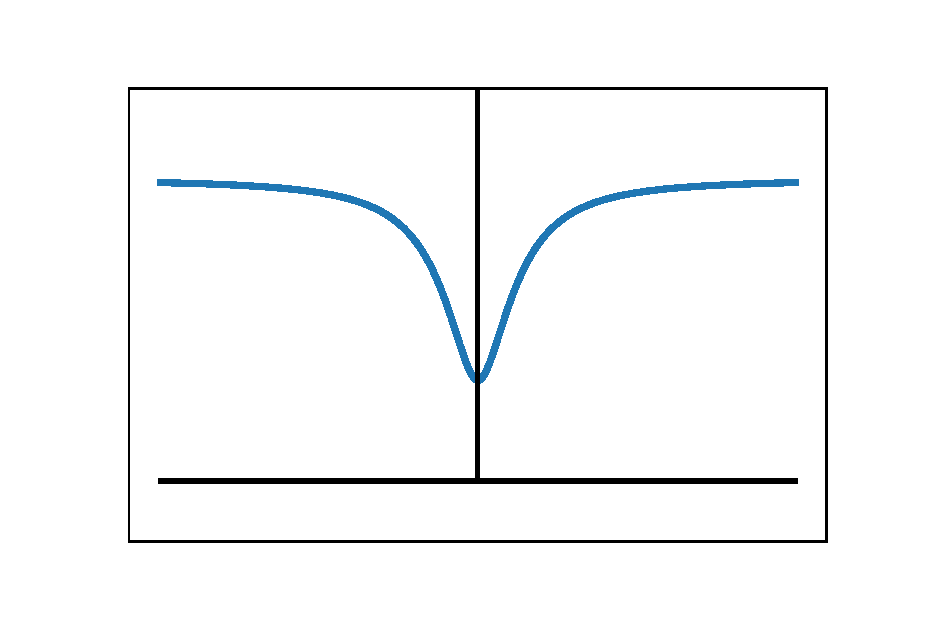
\includegraphics[width=80mm]{PSol10_Q7_zp_3.eps}
\caption{
شکل 3
}
\end{subfigure}
%%%%%%%%%%%%%%%%%%%%%
\begin{subfigure}{0.49\textwidth}
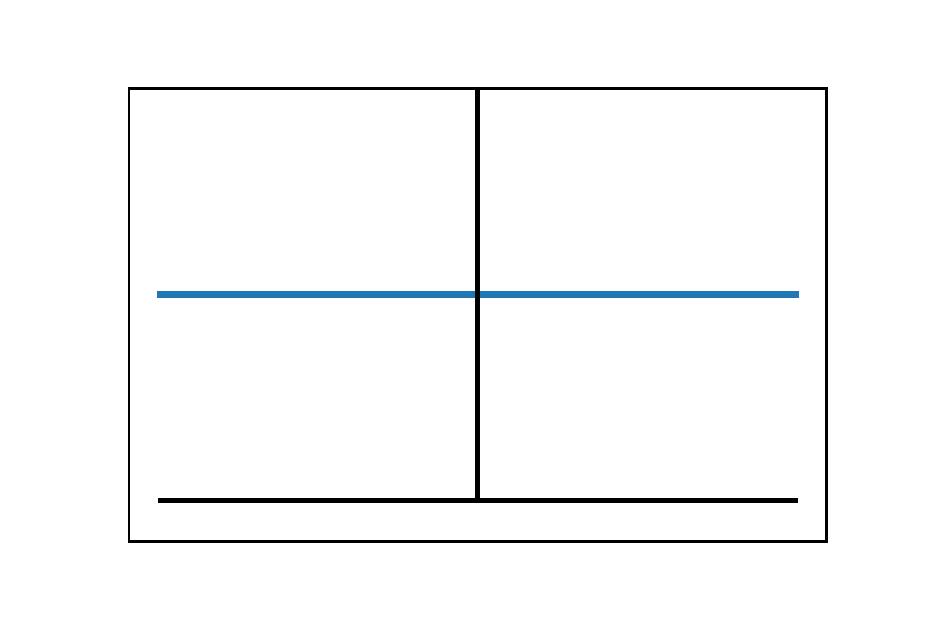
\includegraphics[width=80mm]{PSol10_Q7_zp_4.eps}
\caption{
شکل 4
}
\end{subfigure}
%%%%%%%%%%%%%%%%%%%%%
\end{figure}
\begin{figure}[h!]
\ContinuedFloat
\centering
%%%%%%%%%%%%%%%%%%%%%
\begin{subfigure}{0.49\textwidth}
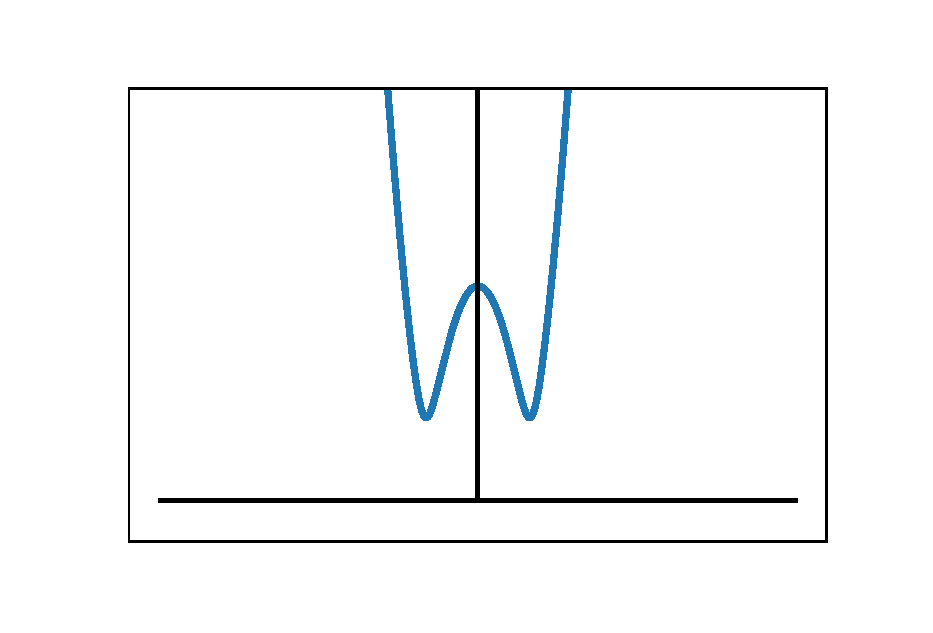
\includegraphics[width=80mm]{PSol10_Q7_zp_5.eps}
\caption{
شکل 5
}
\end{subfigure}
%%%%%%%%%%%%%%%%%%%%%
\begin{subfigure}{0.49\textwidth}
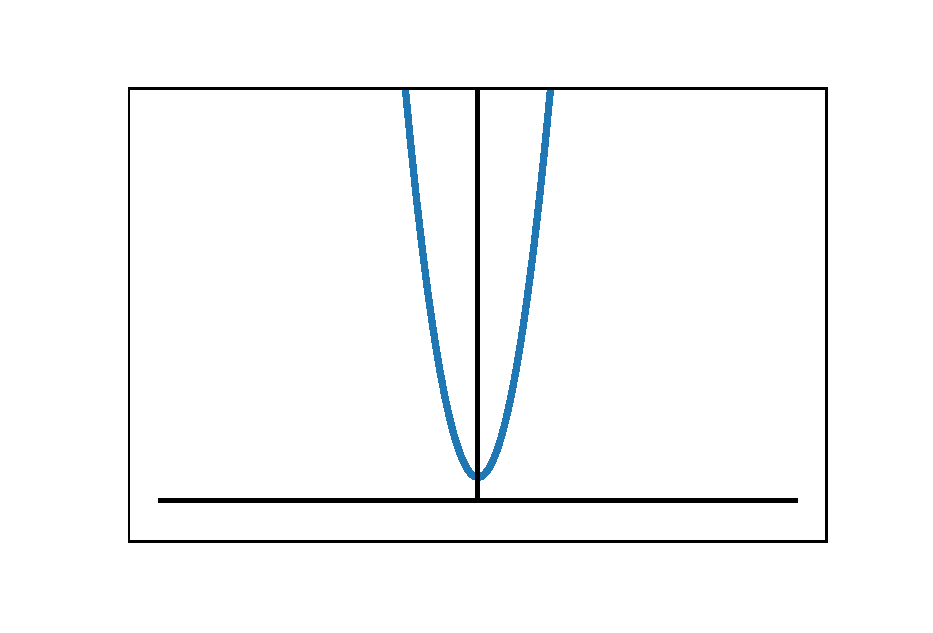
\includegraphics[width=80mm]{PSol10_Q7_zp_6.eps}
\caption{
شکل 6
}
\end{subfigure}
%%%%%%%%%%%%%%%%%%%%%
\end{figure}

\Q

الف)
$$
H(s)={1\over s^2-s-2}={A\over s-2}+{B\over s+1}={{1\over 3}\over s-2}-{{1\over 3}\over s+1}
$$

ب) سیستم پایدار:
$$
h(t)=-{1\over 3}e^{-t}u(t)-{1\over 3}e^{2t}u(-t)
$$
سیستم علی:
$$
h(t)=-{1\over 3}e^{-t}u(t)+{1\over 3}e^{2t}u(t)
$$
سیستم ناپایدار و غیرعلی:
$$
h(t)={1\over 3}e^{-t}u(-t)-{1\over 3}e^{2t}u(-t)
$$

\Q

1.
با توجه به تساوی 
$
[e^s]^*=e^{s^*}
$
 نتیجه می شود:
\qn{
&x(t)\iff X(s)\implies
\\&X(s)=\int_{\Bbb R}x(t)e^{-st}dt\implies
\\&X^*(s)=\int_{\Bbb R}x^*(t)e^{-s^*t}dt\implies
\\&X^*(s^*)=\int_{\Bbb R}x^*(t)e^{-st}dt\implies
\\&x^*(t)\iff X^*(s^*)
}{}
ناحیه همگرایی تغییر نمی کند زیرا تبدیل 
$
s\to s^*
$
، ناحیه همگرایی را نسبت به محور حقیقی قرینه می کند و دوباره همان ناحیه ی پیشین را نتیجه می دهد.

2. 
\qn{
&x(t)={1\over 2\pi j}\int_{\sigma-j\infty}^{\sigma+j\infty} X(s)e^{st}ds\implies
\\&{dx(t)\over dt}={1\over 2\pi j}\int_{\sigma-j\infty}^{\sigma+j\infty} sX(s)e^{st}ds
}{}
ناحیه همگرایی می تواند بزرگتر شود زیرا ضرب شدن تبدیل لاپلاس در $s$، می تواند قطبی را در $s=0$ حذف کند.

3.
\qn{
&x(t)\iff X(s)\implies
\\&X(s)=\int_{\Bbb R}x(t)e^{-st}dt\implies
\\&{d\over ds}X(s)=\int_{\Bbb R}-tx(t)e^{-st}dt\implies
\\&-tx(t)\iff {d\over ds}X(s)
}{}
ناحیه همگرایی تغییر نمی کند؛ زیرا پایداری و علی بودن $x(t)$ با ضرب شدن در $t$ تغییر نمی کند و همچنین قطب های $H(s)$ با قطب های 
$
{d\over ds}X(s)
$
یکسانند.

4.
 می توان گفت 
$
\int_{-\infty}^tx(\tau)d\tau
$
 خروجی سیستمی با ورودی $x(t)$ و پاسخ ضربه‌ی 
$
h(t)=u(t)
$
است؛ پس 
$$
y(t)=x(t)*u(t)
$$
 و باید ناحیه همگرایی تبدیل لاپلاس
$
y(t)
$
شامل اشتراک نواحی همگرایی تبدیل های لاپلاس
$
x(t)
$
 و
$
h(t)=u(t)
$
 باشد که در این صورت خواهیم داشت:
$$
Y(s)=X(s)H(s)={X(s)\over s}\quad,\quad R_\text{جدید}\supset R\cap \left\{s\  : \ \Re\{s\}>0\right\}
$$
\Q

الف) بله؛ زیرا طبق خاصیت 2 سوال قبل، اگر ناحیه همگرایی تبدیل لاپلاس 
$
h(t)
$
شامل محور $j\omega$ و $\infty$ باشد، ناحیه همگرایی تبدیل لاپلاس 
$
{d\over dt}h(t)
$
نیز شامل محور $j\omega$ و $\infty$ خواهد بود.

ب) علی بودن محرز است؛ زیرا به دلیل علی بودن سیستمی با پاسخ $h(t)$ داریم:
$$
\int_{-\infty}^th(\tau)d\tau=\begin{cases}
\int_{0}^th(\tau)d\tau&,\quad t>0\\
0&,\quad t\le 0
\end{cases}
$$
اما ناپایداری الزامی نیست. مثال نقض آن، سیستمی با تابع تبدیل 
$$
H(s)={s\over s+1}\quad,\quad \Re\{s\}>-1
$$
یا پاسخ ضربه‌ی 
$$
h(t)=\delta(t)-e^{-t}u(t)
$$
است که در این صورت سیستمی با پاسخ ضربه‌ی 
$$
\int_{-\infty}^th(\tau)d\tau=e^{-t}u(t)
$$
پایدار و علی خواهد بود.

\Q

الف)
\qn{
X(s)&=\sum_{n=0}^\infty e^{-nT}e^{-nTs}
\\&=\sum_{n=0}^\infty e^{-nT(s+1)}
\\&={1\over 1-e^{-T(s+1)}}
}{}
تساوی اخیر هنگامی برقرار است که :
$$
\Re\{T(s+1)\}>0\implies \Re\{T(s+1)\}>0\implies \Re\{s\}>-1
$$

ب) تبدیل لاپلاس دارای صفر نیست (هیچگاه صفر نمی شود) و برای قطب های آن:
$$
e^{T(s+1)}=1\iff T(s+1)=2jk\pi \iff s={2jk\pi\over T}-1 \quad,\quad k\in\Bbb Z
$$
\begin{figure}[h!]
\centering
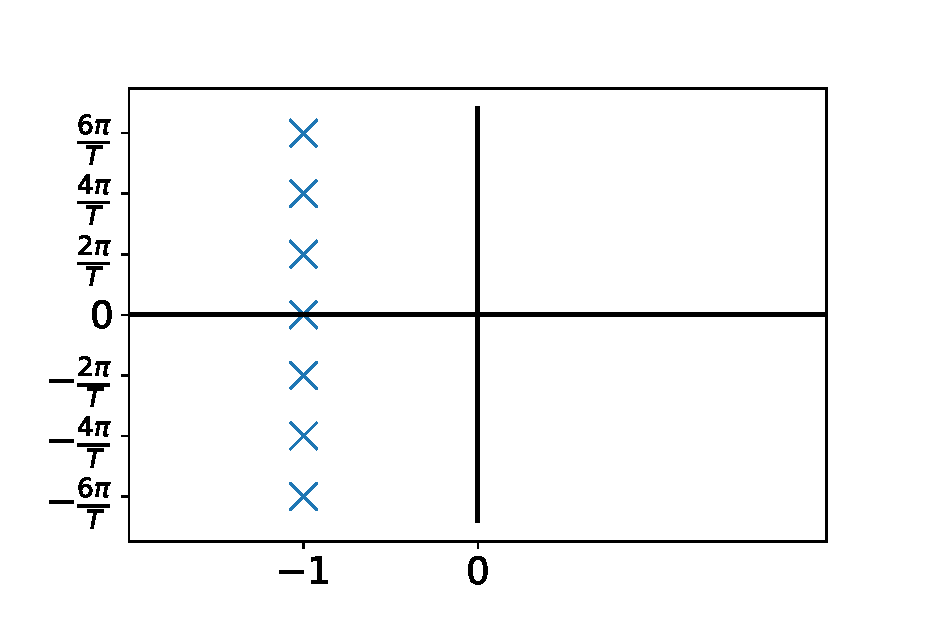
\includegraphics[width=90mm]{PSol11_Q11.eps}
\end{figure}

پ) با ترسیم 
$
|X(j\omega)|
$
خواهیم داشت:
\begin{figure}[h!]
\centering
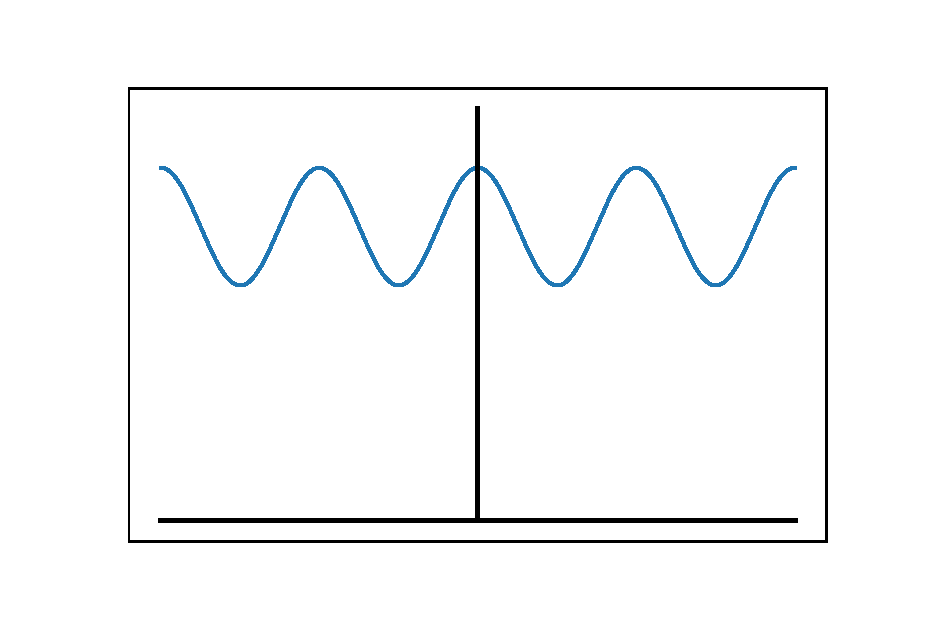
\includegraphics[width=90mm]{PSol11_Q11_2.eps}
\end{figure}

که به وضوح متناوب است.
\end{document}